\chapter{Perturbative Green Functions and Feynman Graphs}
\label{ch:perturbative-green-functions}
\ConventionsMixed


\section{Regulated Euclidean Scalar Theory}

\begin{definition}[Regulated Euclidean \(\phi^4\) datum]
\label{def:regulated-euclidean-phi-four-datum}
Let \(D\ge1\). In this chapter \(x\in\mathbb R^D\) denotes a Euclidean
spacetime point and \(k\in\mathbb R^D\) denotes the corresponding Euclidean
momentum. The field variable is a real scalar function \(\phi\). For the
perturbative Euclidean construction in this chapter, henceforth assume
\(m>0\); this is a stricter infrared convention than the nonnegative invariant
mass parameter allowed in the spectral discussion. The
Lorentzian model whose Green functions are studied perturbatively has classical
density, in the mostly-plus convention,
\[
  \mathcal L
  =
  -\frac{1}{2}\partial_\mu\phi\,\partial^\mu\phi
  -\frac{1}{2}m^2\phi^2
  -\frac{g}{4!}\phi^4 .
\]
The perturbative construction in this chapter is made first for Euclidean
Green functions. Its Euclidean density is
\[
  \mathcal L_E
  =
  \frac{1}{2}(\partial\phi)^2
  +\frac{1}{2}m^2\phi^2
  +\frac{g}{4!}\phi^4 ,
\]
so that the interaction part of the Euclidean action is
\[
  S_{\mathrm{int},E}[\phi]
  =
  \frac{g}{4!}\int\dd^D x\,\phi(x)^4 ,
\]
where \(g\in\mathbb R\) is the quartic coupling.  This expression is a
regulated interaction coordinate.  With the finite-dimensional cutoff
introduced below, \(\phi_\Lambda(x)^4\) is an ordinary function on the regulated
configuration space and the integral is a well-defined polynomial.  The
continuum symbol \(\phi(x)^4\) is not, by itself, a defined local operator:
products of continuum fields at coincident points require a renormalization
prescription.  In this chapter the symbol denotes the regulated monomial
together with the counterterm and renormalization conditions used to define
Green functions order by order.  Renormalized composite insertions, obtained by
coupling local sources and differentiating with respect to renormalized source
coordinates, are constructed later in
Chapter~\ref{ch:volume-ii-renormalized-operators-minimal-subtraction}.

The free covariance is the Euclidean propagator
\[
  \Delta_E(x-y;m^2)
  =
  \int \frac{\dd^D k}{(2\pi)^D}\,
  \frac{\ee^{\ii k\cdot(x-y)}}{k^2+m^2},
\]
with \(m>0\).

The status of the regulator-removal problem depends sharply on \(D\).  For
\(D=2\) and \(D=3\), the renormalized \(\phi^4\) models have constructive
non-Gaussian continuum realizations: in \(D=2\) this belongs to the
\(P(\phi)_2\) construction, and in \(D=3\) the \(\phi^4_3\) construction is
obtained after the required local counterterms.  For the standard
reflection-positive lattice \(\lambda\phi^4\) model with \(\lambda\ge0\) in
\(D=4\), the continuum scaling limits selected by the usual critical or
near-critical tuning are Gaussian.  This is the four-dimensional marginal
triviality theorem completed by the Aizenman--Duminil-Copin analysis, together
with the earlier triviality results of Aizenman and Fr\"ohlich.  The theorem is
a statement about that constructive scaling-limit problem.  The broader
question whether some ultraviolet-complete QFT can have a small-coupling
expansion agreeing with formal \(\phi^4_4\) perturbation theory to all orders
is a separate nonperturbative existence problem.  Thus the four-dimensional
perturbative expansion below should be read as a finite-cutoff and renormalized
asymptotic expansion, and as a valid effective-field-theory expansion below a
cutoff, unless an additional nonperturbative ultraviolet construction is
supplied.

The corresponding constructive question for pure Yang--Mills theory in
\(D=4\) has a different status.  The Clay Millennium problem called
``Yang--Mills existence and mass gap'' asks, for every compact simple gauge
group \(G\), for a continuum quantum Yang--Mills theory on \(\mathbb R^4\)
whose gauge-invariant Schwinger functions satisfy the structural requirements
needed for Euclidean reconstruction and whose reconstructed physical
Hamiltonian has a unique vacuum at energy \(0\) and spectrum contained in
\(\{0\}\cup[\Delta,\infty)\) for some \(\Delta>0\).  Perturbative asymptotic
freedom, lattice regularizations, strong-coupling expansions in finite cutoff
systems, and numerical evidence all belong to the surrounding mathematical and
physical picture; the continuum existence theorem together with the positive
physical mass gap is the open problem.  This is logically distinct from the
\(\phi^4_4\) triviality statement above: the latter is a proved obstruction
for the standard reflection-positive scalar scaling-limit family, while the
former is an open constructive existence and spectral problem for a gauge
theory.

The functional notation is used with a regulator. One concrete choice is a
finite Euclidean box with periodic boundary conditions and only finitely many
Fourier modes retained. Equivalently, in infinite-volume notation, choose a
smooth cutoff function \(\chi_\Lambda(k)\) which is \(1\) for
\(|k|\ll\Lambda\) and rapidly decays for \(|k|\gg\Lambda\), and replace the
free covariance by
\[
  C_\Lambda(x-y)
  =
  \int \frac{\dd^D k}{(2\pi)^D}\,
  \frac{\chi_\Lambda(k)\,\ee^{\ii k\cdot(x-y)}}
  {k^2+m^2}.
\]
At finite regulator the Gaussian expectation \(\vev{\cdots}_{0,\Lambda}\) is
an ordinary finite-dimensional Gaussian expectation, or the limit of such
expectations. Formulas written without \(\Lambda\) are coefficientwise
perturbative formulas or shorthand for regulator-dependent formulas before
the limit is studied.
\end{definition}

\begin{remark}[Constructive status of the scalar example]
The constructive comments above are not used as hidden axioms in the
perturbative derivations below.  They delimit the status of the continuum
limit: every formula in this chapter is first an identity at finite regulator
or a coefficient of a regulated formal power series; the additional question
of removing \(\Lambda\) is a separate renormalization or constructive
existence problem.
\end{remark}

With a sharp Fourier cutoff this finite-dimensional statement is represented
by
\[
  \int[\dd\phi]_\Lambda
  \quad\leadsto\quad
  \int\prod_{|k|\le\Lambda}\dd\widetilde\phi(k),
  \qquad
  \widetilde\phi(-k)=\overline{\widetilde\phi(k)}
\]
after choosing independent real coordinates for one representative of each
pair \(k,-k\) and fixing the resulting finite-dimensional Gaussian
normalization. The symbol \([\dd\phi]\) is never used here as an unregulated
Lebesgue measure on an infinite-dimensional vector space.

\begin{definition}[Normalized regulated Euclidean Green functions]
\label{def:normalized-regulated-euclidean-green-functions}
The normalized Euclidean \(n\)-point function is
\[
\begin{aligned}
  G_{E,n,\Lambda}(x_1,\ldots,x_n)
  &=
  \frac{\vev{
    \phi(x_1)\cdots\phi(x_n)
    \exp[-S_{\mathrm{int},E}[\phi]]
  }_{0,\Lambda}
  }{
  \vev{\exp[-S_{\mathrm{int},E}[\phi]]}_{0,\Lambda}} .
\end{aligned}
\]
It is a distribution in the insertion points after the regulator is removed,
when that limit exists or has been renormalized. Perturbation theory is the
coefficientwise expansion of this expression in powers of the coupling \(g\),
with the regulator kept fixed before renormalized limits are considered.
\end{definition}

\begin{proposition}[Coefficientwise perturbation at fixed regulator]
\label{prop:fixed-regulator-coefficientwise-perturbation}
At any finite regulator for which \(S_{\mathrm{int},E}\) is a polynomial on a
finite-dimensional Gaussian space, the coefficient of \(g^V\) in
\(G_{E,n,\Lambda}\) is obtained by expanding numerator and denominator in
powers of \(S_{\mathrm{int},E}\), taking ordinary Gaussian moments, and then
dividing the resulting formal power series by the denominator series.
\end{proposition}

\begin{proof}
At finite regulator the Gaussian expectation is an ordinary normalized
finite-dimensional integral with positive covariance.  The exponential
\(\exp[-S_{\mathrm{int},E}]\) is treated either as an honest integrable
function for values of \(g\) where the integral converges, or as the formal
series
\[
  \sum_{V\ge0}
  \frac{(-1)^V}{V!}S_{\mathrm{int},E}[\phi]^V .
\]
Since \(S_{\mathrm{int},E}\) is polynomial, each coefficient is a finite sum
of Gaussian moments.  The denominator has constant term \(1\), so it has a
unique inverse as a formal power series in \(g\).  Multiplication by that
inverse gives the displayed normalized Green function coefficient by
coefficient.  No infinite-dimensional measure or regulator-removal operation
enters this algebraic step.
\end{proof}

\section{Wick Expansion and Connected Functions}

\begin{proposition}[Wick graph expansion and connected cumulants]
\label{prop:wick-graph-expansion-connected-cumulants}
For the centered Gaussian expectation,
\[
  \vev{\phi(x_1)\cdots\phi(x_{2r})}_{0,\Lambda}
  =
  \sum_{\text{pairings }P}
  \prod_{\{a,b\}\in P} C_\Lambda(x_a-x_b),
\]
and odd moments vanish. Expanding the interaction gives
\[
\begin{aligned}
  &\vev{
    \phi(x_1)\cdots\phi(x_n)
    \exp[-S_{\mathrm{int},E}[\phi]]
  }_{0,\Lambda}
  \\
  &\quad =
  \sum_{V=0}^\infty
  \frac{(-g)^V}{V!(4!)^V}
  \int \prod_{a=1}^V \dd^D z_a\,
  \vev{
    \phi(x_1)\cdots\phi(x_n)
    \prod_{a=1}^V \phi(z_a)^4
  }_{0,\Lambda}.
\end{aligned}
\]
Each Gaussian moment on the right is a sum over pairings. A pairing is drawn
as an edge; an integration point \(z_a\) is drawn as a four-valent vertex; an
insertion \(x_i\) is an external labelled endpoint. This is the origin of the
Feynman graphs in this chapter.

The denominator in \(G_{E,n,\Lambda}\) cancels components that have no
external endpoint. Therefore a normalized \(n\)-point function is a sum over
graphs whose every connected component contains at least one external label.
The connected \(n\)-point function is the part in which all external labels
belong to one connected component.
\end{proposition}

\begin{proof}
The first displayed formula is Wick's theorem for the finite-dimensional
Gaussian vector obtained by evaluating the regulated field at the indicated
test functions or points.  Substituting the formal exponential expansion of
Proposition~\ref{prop:fixed-regulator-coefficientwise-perturbation} expresses
each coefficient as a finite sum over pairings of the \(n+4V\) field factors.
Every pair in a Wick pairing supplies one covariance \(C_\Lambda\); grouping
the paired half-edges incident to the same interaction point gives precisely
the graph description.

The cancellation of vacuum components is the exponential formula for labelled
structures applied to Wick pairings.  Equivalently, write every pairing graph
as the disjoint union of connected components.  Components with no external
label are generated by the same series that appears in
\(Z_\Lambda[0]\), so division by \(Z_\Lambda[0]\) removes them.  The connected
part is then selected by requiring that the external labels lie in one
component.
\end{proof}

\begin{figure}[H]
\centering
\begin{tikzpicture}[scale=0.9,>=Stealth]
  \fill[blue!10,draw=blue!65!black,very thick] (-1.6,0) ellipse (1.1 and 0.65);
  \fill[blue!10,draw=blue!65!black,very thick] (2.1,0) ellipse (0.95 and 0.55);
  \foreach \p/\lab in {(-2.8,0.5)/x_1,(-2.8,-0.5)/x_2,(3.35,0.45)/x_3,(3.35,-0.45)/x_4} {
    \fill[red!75!black] \p circle (2pt);
    \node[black,above=2pt] at \p {$\lab$};
  }
  \draw[purple!75!black,very thick] (-2.8,0.5)--(-2.1,0.28);
  \draw[purple!75!black,very thick] (-2.8,-0.5)--(-2.1,-0.28);
  \draw[purple!75!black,very thick] (3.35,0.45)--(2.7,0.24);
  \draw[purple!75!black,very thick] (3.35,-0.45)--(2.7,-0.24);
  \node[blue!65!black,align=center,font=\small] at (-1.6,-1.18)
    {external\\component};
  \node[blue!65!black,align=center,font=\small] at (2.1,-1.18)
    {external\\component};
  \draw[orange!80!black,thick,dashed] (0.0,1.25) circle (0.38);
  \node[orange!80!black,align=center,font=\small] at (0.0,2.12)
    {vacuum component\\cancels};
\end{tikzpicture}
\caption{Component selection in normalized Euclidean correlators.  Vacuum
components cancel against the denominator, while every surviving component
contains at least one external insertion.}
\label{fig:normalized-correlator-component-selection}
\end{figure}

\begin{proposition}[Connected Green functions are source cumulants]
\label{prop:connected-green-functions-source-cumulants}
Introduce a source \(J\) and define
\[
  Z_\Lambda[J]
  =
  \vev{
    \exp\left[
      -S_{\mathrm{int},E}[\phi]
      +\int\dd^D x\,J(x)\phi(x)
    \right]
  }_{0,\Lambda}.
\]
The connected generating functional is
\[
  W_\Lambda[J]=\log Z_\Lambda[J].
\]
For \(n\ge1\),
\[
  G^{\mathrm{conn}}_{E,n,\Lambda}(x_1,\ldots,x_n)
  =
  \left.
  \frac{\delta^n W_\Lambda[J]}{
   \delta J(x_1)\cdots\delta J(x_n)}
  \right|_{J=0}.
\]
This identity is the cumulant identity for the regulated probability measure.
\end{proposition}

\begin{proof}
At finite regulator \(Z_\Lambda[J]\) is the moment generating functional of a
finite-dimensional random vector after adjoining the polynomial weight
\(\exp[-S_{\mathrm{int},E}]\).  The logarithm of a moment generating function
is the cumulant generating function.  Differentiating \(W_\Lambda[J]\) at
\(J=0\) therefore gives the joint cumulant of the \(n\) inserted fields.  The
moment-cumulant relation is equivalent to the connected-component expansion of
the preceding proposition, so the functional derivatives of \(W_\Lambda\) are
exactly the connected regulated Green functions.
\end{proof}

\section{Momentum-Space Graph Weights}

\begin{definition}[Euclidean graph weight]
\label{def:momentum-space-labelled-euclidean-graph-weight}
In translation-invariant infinite-volume notation, write
\[
  G_{E,n}^{\mathrm{conn}}(x_1,\ldots,x_n)
  =
  \int \prod_{i=1}^n \frac{\dd^D k_i}{(2\pi)^D}\,
  \ee^{\ii\sum_i k_i\cdot x_i}\,
  \widetilde G_{E,n}^{\mathrm{conn}}(k_1,\ldots,k_n).
\]
A connected graph \(\Gamma\) with labelled external legs contributes a
distribution of the form
\[
  \mathcal A_E(\Gamma;k_1,\ldots,k_n)
  =
  (2\pi)^D\delta^{(D)}\!\left(\sum_{i=1}^n k_i\right)
  I_E(\Gamma;k_1,\ldots,k_n).
\]
The reduced integrand \(I_E\) is computed as follows. Assign momentum to every
edge, impose momentum conservation at every vertex, integrate over one
independent momentum for each loop, and multiply by
\[
  \frac{(-g)^{V(\Gamma)}}{|\operatorname{Aut}\Gamma|}
  \prod_{e\in E(\Gamma)}
  \frac{1}{p_e^2+m^2}.
\]
Here \(V(\Gamma)\) is the number of quartic vertices, \(E(\Gamma)\) is the set
of internal and external propagator edges, \(p_e\) is the momentum carried by
edge \(e\), and \(\operatorname{Aut}\Gamma\) is the group of graph
automorphisms preserving all external labels. This convention includes the
factor \(1/4!\) in the action and the Wick-contraction multiplicities in the
single symmetry factor.
\end{definition}

\begin{figure}[H]
\centering
\begin{tikzpicture}[scale=0.9,>=Stealth]
  \draw[very thick,->] (-1.25,0)--(1.25,0) node[midway,above] {$k$};
  \node at (2.0,0) {$=$};
  \node at (3.25,0) {$\displaystyle \frac{1}{k^2+m^2}$};

  \begin{scope}[xshift=7.0cm]
    \fill[blue!80!black] (0,0) circle (2.5pt);
    \foreach \ang/\lab in {135/k_1,45/k_2,-45/k_3,-135/k_4} {
      \draw[very thick,->] ({1.0*cos(\ang)},{1.0*sin(\ang)}) -- (0,0);
      \node at ({1.34*cos(\ang)},{1.34*sin(\ang)}) {$\lab$};
    }
    \node at (1.85,0) {$=$};
    \node[align=left,anchor=west] at (2.25,0)
      {$\displaystyle -g\,(2\pi)^D
        \delta^{(D)}(k_1+k_2+k_3+k_4)$};
  \end{scope}
\end{tikzpicture}
\caption{Momentum-space Feynman rules for Euclidean \(\phi^4\) theory with
labelled external legs.  The propagator is \((k^2+m^2)^{-1}\), and the quartic
vertex includes momentum conservation.}
\label{fig:euclidean-phi-four-feynman-rules}
\end{figure}

The displayed vertex rule is the labelled-leg rule. If instead one expands
directly from the action, each vertex gives \(-g/4!\) and the \(4!\) is
recovered by counting Wick contractions.

\section{Symmetry Factors from Wick Pairings}

\begin{proposition}[Automorphism denominator from Wick pairings]
\label{prop:automorphism-denominator-from-wick-pairings}
The coefficient \( |\operatorname{Aut}\Gamma|^{-1} \) in the graph rule is
the residual count left by the regulated Wick expansion. Consider a connected
graph \(\Gamma\) with \(V\) quartic
vertices and labelled external endpoints. Let
\(\operatorname{Aut}\Gamma\) denote the automorphism group preserving the
external labels and the incidence relation between vertices and half-edges.
The \(V\)-th term of the interaction expansion carries the prefactor
\[
  \frac{(-g)^V}{V!(4!)^V}.
\]
If the abstract graph \(\Gamma\) is fixed, the number of choices of ordered
interaction vertices, ordered half-edges at each vertex, and Wick pairings
which realize this same labelled graph is
\[
  \frac{V!(4!)^V}{|\operatorname{Aut}\Gamma|}.
\]
Multiplying the two factors gives precisely
\[
  \frac{(-g)^V}{|\operatorname{Aut}\Gamma|}.
\]
Thus the graph automorphism factor is the quotient between the arbitrary
labellings introduced by the expansion and the relabellings leaving the graph
unchanged.
\end{proposition}

\begin{proof}
Start with the \(V\)-th term of the regulated expansion, where the integration
variables \(z_1,\ldots,z_V\) are ordered and the four field factors at each
vertex are ordered by their position in \(\phi(z_a)^4\).  These choices give
\(V!(4!)^V\) auxiliary labels for the same abstract incidence graph.  The
Wick pairing then identifies half-edges in pairs to form internal edges or
connects half-edges to the fixed external labels.  For a fixed labelled
external graph \(\Gamma\), the group
\(\operatorname{Aut}\Gamma\) is exactly the stabilizer of this labelling data:
it consists of the vertex and half-edge relabellings that leave the incidence
relations and all external labels unchanged.  By the orbit-stabilizer
identity, the number of labelled Wick contractions giving the same abstract
\(\Gamma\) is \(V!(4!)^V/|\operatorname{Aut}\Gamma|\).  Multiplying by the
expansion prefactor gives \((-g)^V/|\operatorname{Aut}\Gamma|\).
\end{proof}

For example, the order-\(g\) tadpole correction to the two-point function has
one quartic vertex. The two external labels are fixed, while the two remaining
half-edges form the loop and may be interchanged. Hence
\(|\operatorname{Aut}\Gamma|=2\), and the coefficient is \(-g/2\). In the
unlabelled-vertex convention this same count is
\[
  \left(-\frac{g}{4!}\right)
  \left(4\cdot3\cdot\frac{2!}{2}\right)
  =
  -\frac{g}{2}.
\]
Here the \(4\) chooses the vertex half-edge contracted with the first external
endpoint, and the \(3\) chooses the half-edge contracted with the second
external endpoint.  The remaining two half-edges form the loop.  If they are
temporarily ordered this gives a factor \(2!\), and the quotient by \(2\)
identifies the interchange of the two ends of the same loop, leaving one loop
pairing.

For the two-vertex sunset insertion in the two-point function, the expansion
prefactor and the Wick-pairing count give
\[
  \frac{1}{2!}
  \left(-\frac{g}{4!}\right)^2
  \left(2\cdot4^2\cdot3!\right)
  =
  4\cdot4!\left(-\frac{g}{4!}\right)^2
  =
  \frac{g^2}{6}.
\]
The first factor \(2\) assigns the two external endpoints to the two
interaction vertices, each \(4\) chooses the external half-edge at one vertex,
and \(3!\) pairs the remaining half-edges between the vertices. The single
quartic contribution to the connected four-point function with four labelled
external insertions has trivial automorphism group, and its coefficient is
\(-g\). Vacuum components have already been removed by normalization; the
logarithm of the generating functional then selects the component in which all
external labels are connected.

\section{Two-Point Function and Self-Energy}

The connected Euclidean two-point function has Fourier transform
\[
  G_E(x,y)
  =
  \int \frac{\dd^D k}{(2\pi)^D}\,
  \ee^{\ii k\cdot(x-y)}\,\widetilde G_E(k).
\]
Its perturbative expansion begins as
\[
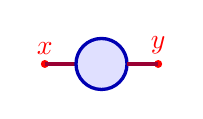
\begin{tikzpicture}[baseline=-0.45ex,scale=0.72]
  \fill[red] (-1,0) circle (2pt) node[above] {$x$};
  \fill[red] (1,0) circle (2pt) node[above] {$y$};
  \draw[purple!80!black,very thick] (-1,0)--(-0.45,0);
  \fill[blue!12,draw=blue!70!black,very thick] (0,0) circle (0.45);
  \draw[purple!80!black,very thick] (0.45,0)--(1,0);
\end{tikzpicture}
\quad=\quad
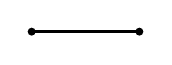
\begin{tikzpicture}[baseline=-0.45ex,scale=0.72]
  \fill (-0.95,0) circle (2pt);
  \fill (0.95,0) circle (2pt);
  \draw[very thick] (-0.95,0)--(0.95,0);
\end{tikzpicture}
\quad+\quad
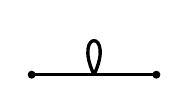
\begin{tikzpicture}[baseline=-0.45ex,scale=0.72]
  \fill (-1.1,0) circle (2pt);
  \fill (1.1,0) circle (2pt);
  \draw[very thick] (-1.1,0)--(1.1,0);
  \draw[very thick] (0,0) .. controls (-0.38,0.8) and (0.38,0.8) .. (0,0);
\end{tikzpicture}
\quad+\quad
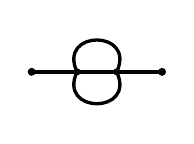
\begin{tikzpicture}[baseline=-0.45ex,scale=0.72]
  \fill (-1.15,0) circle (2pt);
  \fill (1.15,0) circle (2pt);
  \draw[very thick] (-1.15,0)--(1.15,0);
  \fill (-0.35,0) circle (1.8pt);
  \fill (0.35,0) circle (1.8pt);
  \draw[very thick] (-0.35,0) .. controls (-0.7,0.75) and (0.7,0.75) .. (0.35,0);
  \draw[very thick] (-0.35,0) .. controls (-0.7,-0.75) and (0.7,-0.75) .. (0.35,0);
\end{tikzpicture}
\quad+\cdots .
\]

\begin{definition}[Euclidean self-energy]
\label{def:euclidean-self-energy}
Define the Euclidean self-energy \(\Sigma_E(k)\) by the Dyson form
\begin{equation}
  \widetilde G_E(k)
  =
  \frac{1}{k^2+m^2-\Sigma_E(k)} .
  \label{eq:euclidean-self-energy}
\end{equation}
Equivalently,
\[
  \widetilde G_E
  =
  G_{0,E}
  +
  G_{0,E}\Sigma_E G_{0,E}
  +
  G_{0,E}\Sigma_E G_{0,E}\Sigma_E G_{0,E}
  +\cdots,
  \qquad
  G_{0,E}(k)=\frac{1}{k^2+m^2}.
\]
With this sign convention \(\Sigma_E\) is the sum of amputated connected
one-particle-irreducible two-point insertions.
\end{definition}

\[
\Sigma_E(k)
=
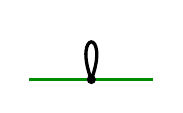
\begin{tikzpicture}[baseline=-0.45ex,scale=0.75]
  \draw[green!55!black,very thick] (-1.05,0)--(1.05,0);
  \fill (0,0) circle (2.2pt);
  \draw[very thick] (0,0) .. controls (-0.32,0.85) and (0.32,0.85) .. (0,0);
\end{tikzpicture}
\quad+\quad
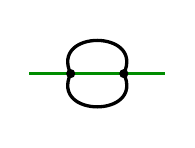
\begin{tikzpicture}[baseline=-0.45ex,scale=0.75]
  \draw[green!55!black,very thick] (-1.15,0)--(1.15,0);
  \fill (-0.45,0) circle (2.2pt);
  \fill (0.45,0) circle (2.2pt);
  \draw[very thick] (-0.45,0) .. controls (-0.8,0.75) and (0.8,0.75) .. (0.45,0);
  \draw[very thick] (-0.45,0) .. controls (-0.8,-0.75) and (0.8,-0.75) .. (0.45,0);
\end{tikzpicture}
\quad+\quad
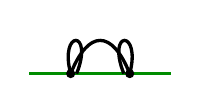
\begin{tikzpicture}[baseline=-0.45ex,scale=0.75]
  \draw[green!55!black,very thick] (-1.2,0)--(1.2,0);
  \fill (-0.5,0) circle (2.2pt);
  \fill (0.5,0) circle (2.2pt);
  \draw[very thick] (-0.5,0) .. controls (-0.7,0.75) and (-0.1,0.75) .. (-0.4,0);
  \draw[very thick] (-0.5,0) .. controls (-0.2,0.75) and (0.2,0.75) .. (0.5,0);
  \draw[very thick] (0.5,0) .. controls (0.7,0.75) and (0.1,0.75) .. (0.4,0);
\end{tikzpicture}
\quad+\cdots .
\]

\begin{proposition}[One-loop tadpole self-energy and cutoff growth]
\label{prop:one-loop-tadpole-self-energy-cutoff-growth}
The order-\(g\) tadpole is
\[
\begin{tikzpicture}[baseline=-0.45ex,scale=0.75,>=Stealth]
  \draw[green!55!black,very thick,->] (-1.1,0)--(0,0) node[midway,below] {$k$};
  \draw[green!55!black,very thick,->] (1.1,0)--(0,0) node[midway,below] {$k$};
  \fill (0,0) circle (2.2pt);
  \draw[very thick,->] (0,0) .. controls (-0.35,0.9) and (0.35,0.9) .. (0,0)
    node[midway,above] {$q$};
\end{tikzpicture}
\quad=\quad
-\frac{g}{2}
\int \frac{\dd^D q}{(2\pi)^D}\,\frac{1}{q^2+m^2}.
\]
The factor \(1/2\) is the symmetry factor of the tadpole graph. This insertion
is independent of the external momentum \(k\), because no external momentum
flows through the closed loop. In the continuum notation the loop integral is
ultraviolet divergent for \(D\ge2\). With a sharp momentum cutoff used only to
display the degree of divergence,
\[
  C_1(\Lambda,m)
  =
  \frac{1}{2}
  \int_{|q|\le\Lambda}
  \frac{\dd^D q}{(2\pi)^D}\,\frac{1}{q^2+m^2}
\]
equals
\[
  \frac{1}{2}
  \frac{\operatorname{vol}(S^{D-1})}{(2\pi)^D}
  \int_0^\Lambda \dd r\,\frac{r^{D-1}}{r^2+m^2},
  \qquad
  \operatorname{vol}(S^{D-1})
  =
  \frac{2\pi^{D/2}}{\Gamma(D/2)}.
\]
Thus
\[
  C_1(\Lambda,m)
  \sim
  \begin{cases}
    \dfrac{1}{4\pi}\log\dfrac{\Lambda}{m}, & D=2,\\[2mm]
    \dfrac{1}{2}
    \dfrac{\operatorname{vol}(S^{D-1})}{(2\pi)^D}
    \dfrac{\Lambda^{D-2}}{D-2}, & D\ge3,
  \end{cases}
\]
up to finite terms and convention-dependent cutoff terms.  The first line uses
\[
  \int_0^\Lambda
  \frac{r\,\dd r}{r^2+m^2}
  =
  \frac{1}{2}\log\frac{\Lambda^2+m^2}{m^2}
  =
  \log\frac{\Lambda}{m}+O(\Lambda^{-2})
\]
inside the radial expression. The second line uses
\(r^{D-1}(r^2+m^2)^{-1}=r^{D-3}+O(r^{D-5})\) at large \(r\).  Hence
\[
  \Sigma_E^{(1)}(k)=-g\,C_1(\Lambda,m).
\]
\end{proposition}

\begin{proof}
The coefficient \(-g/2\) is the symmetry factor computed in
Proposition~\ref{prop:automorphism-denominator-from-wick-pairings}: the two
unattached half-edges at the quartic vertex form one loop and may be
interchanged.  No external momentum enters the loop propagator, so the
amputated insertion is momentum independent and equals the displayed
regulated integral.  In spherical coordinates the cutoff integral is
\[
  \frac12
  \frac{\operatorname{vol}(S^{D-1})}{(2\pi)^D}
  \int_0^\Lambda \frac{r^{D-1}\,\dd r}{r^2+m^2}.
\]
For \(D=2\) the integral is
\(\frac12\log((\Lambda^2+m^2)/m^2)=\log(\Lambda/m)+O(\Lambda^{-2})\).
For \(D\ge3\), subtract the leading asymptotic term
\(r^{D-3}\); the remainder is lower degree at infinity, so the leading
growth is \(\Lambda^{D-2}/(D-2)\) with the displayed prefactor.  The Dyson
sign convention of Definition~\ref{def:euclidean-self-energy} then gives
\(\Sigma_E^{(1)}=-gC_1\).
\end{proof}

\begin{proposition}[Two-loop sunset insertion]
\label{prop:two-loop-sunset-insertion}
The order-\(g^2\) sunset insertion is
\[
\begin{aligned}
\begin{tikzpicture}[baseline=-0.45ex,scale=0.72,>=Stealth]
  \draw[green!55!black,very thick,->] (-1.35,0)--(-0.55,0) node[midway,below] {$k$};
  \draw[green!55!black,very thick,->] (1.35,0)--(0.55,0) node[midway,below] {$k$};
  \fill (-0.55,0) circle (2.2pt);
  \fill (0.55,0) circle (2.2pt);
  \draw[very thick,->] (-0.55,0) .. controls (-0.8,0.8) and (0.8,0.8) .. (0.55,0)
    node[midway,above] {$q_1$};
  \draw[very thick,->] (-0.55,0)--(0.55,0) node[midway,above] {$q_2$};
  \draw[very thick,->] (-0.55,0) .. controls (-0.8,-0.8) and (0.8,-0.8) .. (0.55,0)
    node[midway,below] {$k-q_1-q_2$};
\end{tikzpicture}
&=
\frac{g^2}{6}
\int \frac{\dd^D q_1\,\dd^D q_2}{(2\pi)^{2D}}
\\[-1mm]
&\quad\times
\frac{1}{
  (q_1^2+m^2)(q_2^2+m^2)
  \bigl((k-q_1-q_2)^2+m^2\bigr)} .
\end{aligned}
\]
This formula is a Euclidean integral.  Its Lorentzian boundary values are
obtained by analytic continuation with contour-deformation control; for
timelike external momentum the three-particle Landau threshold of this graph
prevents a naive independent Wick rotation of the loop energies.
\end{proposition}

\begin{proof}
The graph has two quartic vertices and three internal lines joining them.
After the two external half-edges are fixed, the remaining three internal
edges may be permuted, giving the automorphism factor \(3!\).  Thus the
coefficient is \(g^2/6\), in agreement with the Wick-pairing count in the
preceding section.  Momentum conservation at the two vertices leaves two
independent loop momenta, chosen as \(q_1,q_2\); the third internal momentum
is then \(k-q_1-q_2\).  Multiplication of the three Euclidean propagators gives
the displayed integral.  The final statement follows because the Euclidean
integral is defined on real \(D\)-momenta, while Lorentzian boundary values are
obtained by continuing external energy and deforming loop-energy contours
without crossing singularities.  At the three-particle threshold the Landau
equations allow simultaneous on-shell internal lines, so this deformation
cannot be represented as an independent rotation of each loop energy.
\end{proof}

\section{Pole Mass and Counterterm Bookkeeping}

\begin{definition}[Pole mass of an interpolating scalar field]
\label{def:pole-mass-interpolating-scalar-field}
As derived in Chapter~\ref{ch:kallen-lehmann}, the spectral representation of
the Euclidean two-point function has the form
\[
  \widetilde G_E(k)
  =
  \frac{Z}{k^2+m_*^2}
  +
  \int_{[0,\infty)}
  \frac{\dd\rho_{\mathrm c}(s)}{k^2+s},
\]
with an isolated atom at \(s=m_*^2\) when the chosen field has nonzero overlap
with a stable one-particle state. The parameter \(m_*\) is the pole mass read
from the two-point function. Equivalently, singularities of the Euclidean
function in the complex \(k^2\)-plane lie at \(k^2=-s\), and an isolated
one-particle state gives the nearest such pole when no lighter state couples to
the field. At fixed spatial momentum, the same pole appears in the complex
Euclidean energy plane at
\[
  k_D=\pm\ii\sqrt{\vec k^{\,2}+m_*^2}.
\]

The field variable \(\phi\) appearing in the regulated Lagrangian and in the
source \(J\) is the perturbative representative of an interpolating local
field.  Its renormalized two-point function is the full function
\(\widetilde G_E(k)\), with pole residue \(Z\) and continuum spectral
contributions.  The asymptotic scalar field used in scattering theory is the
free field on the isolated one-particle asymptotic Fock space with pole mass
\(m_*\) and unit residue.  Perturbation theory in this chapter locates the pole
and residue of the interpolating-field Green function; the LSZ theorem later
uses those data to project external legs onto the asymptotic one-particle
states.
\end{definition}

\begin{proposition}[One-loop pole shift and mass-coordinate prescription]
\label{prop:one-loop-pole-shift-mass-coordinate-prescription}
Using
\[
  \widetilde G_E(k)
  =
  \frac{1}{k^2+m^2-\Sigma_E(k)}
\]
and the tadpole value above, the pole position satisfies, to first order,
\[
  m_*^2=m^2+gC_1(\Lambda,m)+O(g^2)
\]
in this cutoff scheme. The parameter \(m\) is therefore a parameter of the
regulated quadratic action. Its relation to the spectral pole mass depends on
the regulator and on the prescription used to define the finite theory.
At fixed regulator, \(g\) is a bookkeeping parameter for the coefficientwise
expansion. The coefficient \(C_1(\Lambda,m)\) grows with the cutoff in
\(D\ge2\), so the product \(gC_1(\Lambda,m)\) is not uniformly small as
\(\Lambda\to\infty\). Thus the distinction between a cutoff-dependent
quadratic action coordinate and a mass defined by spectral data is
operational in the cutoff-dependent calculation.

A perturbative mass prescription introduces a renormalized parameter \(m_R\)
and a counterterm \(\delta m^2\):
\[
  m^2=m_R^2+\delta m^2,
  \qquad
  \delta m^2=\sum_{r\ge1}g^r(\delta m^2)^{(r)}.
\]
The Euclidean Lagrangian density is written as
\[
  \mathcal L_E
  =
  \frac{1}{2}(\partial\phi)^2
  +\frac{1}{2}m_R^2\phi^2
  +\frac{g}{4!}\phi^4
  +\frac{1}{2}\delta m^2\phi^2.
\]
The counterterm coefficient is part of this same regulated Lagrangian, written
in the renormalized coordinate \(m_R\).  In perturbative bookkeeping it is
treated as part of the interaction. At order \(g\), the two-valent
counterterm vertex contributes
\[

\begin{tikzpicture}[baseline=-0.45ex,scale=0.85]
  \draw[purple!80!black,very thick] (-1,0)--(1,0);
  \fill[blue!80!black] (0,0) circle (2.4pt);
\end{tikzpicture}
\qquad\longleftrightarrow\qquad
-(\delta m^2)^{(1)}g .
\]
The condition \(m_*=m_R+O(g^2)\), written at the level of squared masses,
requires
\[
  (\delta m^2)^{(1)}
  =
  -C_1(\Lambda,m_R)+\text{finite prescription term}.
\]
Different finite terms correspond to different renormalization prescriptions.
The split into \(m_R^2\) and \(\delta m^2\) is a prescription-dependent
reorganization of the regulated perturbative calculation. Its role is to make
the cancellation of cutoff-dependent local terms occur coefficient by
coefficient in the expansion in \(g\). The physical statement is made after
Green functions are expressed in terms of the chosen finite parameters, such as
the pole mass \(m_*\). In the on-shell mass prescription the finite terms are
chosen so that \(m_R=m_*\) order by order.
\end{proposition}

\begin{proof}
To first order, insert
\(\Sigma_E^{(1)}(k)=-gC_1(\Lambda,m)\) from
Proposition~\ref{prop:one-loop-tadpole-self-energy-cutoff-growth} into the
Dyson denominator:
\[
  k^2+m^2-\Sigma_E(k)
  =
  k^2+m^2+gC_1(\Lambda,m)+O(g^2).
\]
The pole in the variable \(k^2\) is therefore at
\(k^2=-m^2-gC_1(\Lambda,m)+O(g^2)\), equivalently
\(m_*^2=m^2+gC_1(\Lambda,m)+O(g^2)\).  If the quadratic coordinate of the
regulated action is rewritten as \(m_R^2+\delta m^2\), the counterterm is a
two-valent interaction vertex with the sign displayed above.  Requiring the
pole to sit at \(m_R^2\) through order \(g\) forces the order-\(g\) part of
\(\delta m^2\) to cancel \(C_1(\Lambda,m_R)\), up to the chosen finite
renormalization convention.
\end{proof}

\section{Connected Four-Point Function}

\begin{proposition}[Four-point moment-cumulant decomposition]
\label{prop:four-point-moment-cumulant-decomposition}
For four insertions, the normalized Green function decomposes into pairwise
products of two-point functions and a connected part:
\[
\begin{aligned}
  &G_{E,4}(x_1,x_2,x_3,x_4)
  \\
  &\quad =
  G_E(x_1,x_2)G_E(x_3,x_4)
  +G_E(x_1,x_3)G_E(x_2,x_4)
  +G_E(x_1,x_4)G_E(x_2,x_3)
  \\
  &\qquad
  +G_{E,4}^{\mathrm{conn}}(x_1,x_2,x_3,x_4).
\end{aligned}
\]
\end{proposition}

\begin{proof}
Apply the moment-cumulant identity to four fields.  If the theory is
\(\mathbb Z_2\)-invariant, as the regulated \(\phi^4\) theory is, all odd
cumulants vanish.  The partitions of four labels therefore contribute either
one four-label cumulant or one of the three partitions into two pairs.  The
pair cumulants are the full two-point functions \(G_E\), and the four-label
cumulant is, by definition, \(G_{E,4}^{\mathrm{conn}}\).
\end{proof}

\begin{figure}[H]
\centering
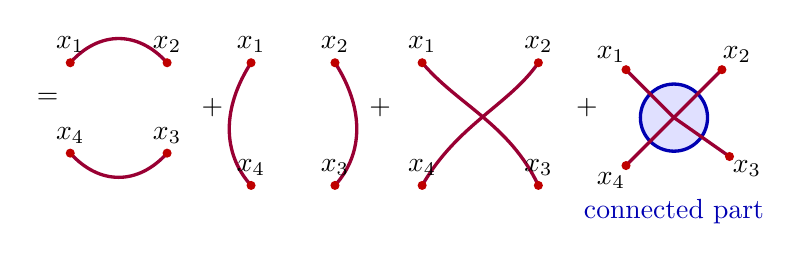
\begin{tikzpicture}[scale=0.82]
  \node at (-0.35,1.2) {$=$};
  \draw[purple!80!black,very thick] (0,1.75) .. controls (0.45,2.25) and (1.05,2.25) .. (1.5,1.75);
  \draw[purple!80!black,very thick] (0,0.35) .. controls (0.45,-0.15) and (1.05,-0.15) .. (1.5,0.35);
  \foreach \p/\lab in {(0,1.75)/x_1,(1.5,1.75)/x_2,(1.5,0.35)/x_3,(0,0.35)/x_4} {
    \fill[red!75!black] \p circle (2pt);
    \node[above] at \p {$\lab$};
  }

  \node at (2.2,1.05) {$+$};
  \draw[purple!80!black,very thick] (2.8,1.75) .. controls (2.35,1.05) and (2.35,0.35) .. (2.8,-0.15);
  \draw[purple!80!black,very thick] (4.1,1.75) .. controls (4.55,1.05) and (4.55,0.35) .. (4.1,-0.15);
  \foreach \p/\lab in {(2.8,1.75)/x_1,(4.1,1.75)/x_2,(4.1,-0.15)/x_3,(2.8,-0.15)/x_4} {
    \fill[red!75!black] \p circle (2pt);
    \node[above] at \p {$\lab$};
  }

  \node at (4.8,1.05) {$+$};
  \draw[purple!80!black,very thick] (5.45,1.75) .. controls (6.0,1.1) and (6.8,0.8) .. (7.25,-0.15);
  \draw[purple!80!black,very thick] (7.25,1.75) .. controls (6.8,1.1) and (6.0,0.8) .. (5.45,-0.15);
  \foreach \p/\lab in {(5.45,1.75)/x_1,(7.25,1.75)/x_2,(7.25,-0.15)/x_3,(5.45,-0.15)/x_4} {
    \fill[red!75!black] \p circle (2pt);
    \node[above] at \p {$\lab$};
  }

  \node at (8.0,1.05) {$+$};
  \fill[blue!12,draw=blue!70!black,very thick] (9.35,0.9) circle (0.52);
  \foreach \ang/\lab in {135/x_1,45/x_2,-35/x_3,-135/x_4} {
    \draw[purple!80!black,very thick]
      (9.35,0.9) -- ({9.35+1.05*cos(\ang)},{0.9+1.05*sin(\ang)});
    \fill[red!75!black] ({9.35+1.05*cos(\ang)},{0.9+1.05*sin(\ang)}) circle (2pt);
    \node at ({9.35+1.38*cos(\ang)},{0.9+1.38*sin(\ang)}) {$\lab$};
  }
  \node[blue!70!black] at (9.35,-0.55) {connected part};
\end{tikzpicture}
\caption{Disconnected and connected parts of the Euclidean four-point function.
The three Wick pairings are separated from
\(G_{E,4}^{\mathrm{conn}}\).}
\label{fig:four-point-wick-connected-decomposition}
\end{figure}

\begin{proposition}[Leading connected four-point Green function]
\label{prop:leading-connected-four-point-green-function}
The Fourier transform of the connected part is defined by
\[
\begin{aligned}
  G_{E,4}^{\mathrm{conn}}(x_1,\ldots,x_4)
  &=
  \int
  \prod_{i=1}^4 \frac{\dd^D k_i}{(2\pi)^D}\,
  \ee^{\ii\sum_i k_i\cdot x_i}\,
  \widetilde G_{E,4}^{\mathrm{conn}}(k_1,\ldots,k_4).
\end{aligned}
\]
To leading order,
\[
\begin{aligned}
  \widetilde G_{E,4}^{\mathrm{conn}}(k_1,\ldots,k_4)
  &=
  (2\pi)^D\delta^{(D)}(k_1+k_2+k_3+k_4)
  \\
  &\quad\times
  \left[
    -g\prod_{i=1}^4 \frac{1}{k_i^2+m^2}
    +O(g^2)
  \right].
\end{aligned}
\]
This is a connected Green function with external propagators included. Later,
after scattering states and LSZ have been constructed, the operation of
removing the external propagators will acquire its scattering interpretation.
\end{proposition}

\begin{proof}
The order-\(g\) connected four-point graph has one quartic vertex and four
labelled external endpoints.  The \(1/4!\) in the interaction is cancelled by
the \(4!\) assignments of the four labelled external fields to the four
half-edges of the vertex, so the vertex coefficient is \(-g\).  Translation
invariance supplies the momentum-conserving delta function.  Each external
field remains connected to the vertex by a Euclidean free propagator, giving
\(\prod_i(k_i^2+m^2)^{-1}\).  Since this is a Green function rather than an
amputated scattering amplitude, those external propagators are part of the
coefficient.
\end{proof}
